%\documentclass{cumcmthesis}
\documentclass[withoutpreface,bwprint]{cumcmthesis} %去掉封面与编号页,电子版提交的时候使用。
\usepackage[final]{pdfpages}
\usepackage[linesnumbered,boxed,ruled,commentsnumbered]{algorithm2e}
\usepackage[framemethod=TikZ]{mdframed}
\usepackage{url}   % 网页链接
\usepackage{subcaption} % 子标题
\title{}
\tihao{A}
\baominghao{}
\schoolname{杭州电子科技大学}
\membera{ }
\memberb{ }
\memberc{ }
\supervisor{ }
\yearinput{2020}
\monthinput{08}
\dayinput{22}
\renewcommand\thesection{\arabic{section}.}

\begin{document}
	
	
	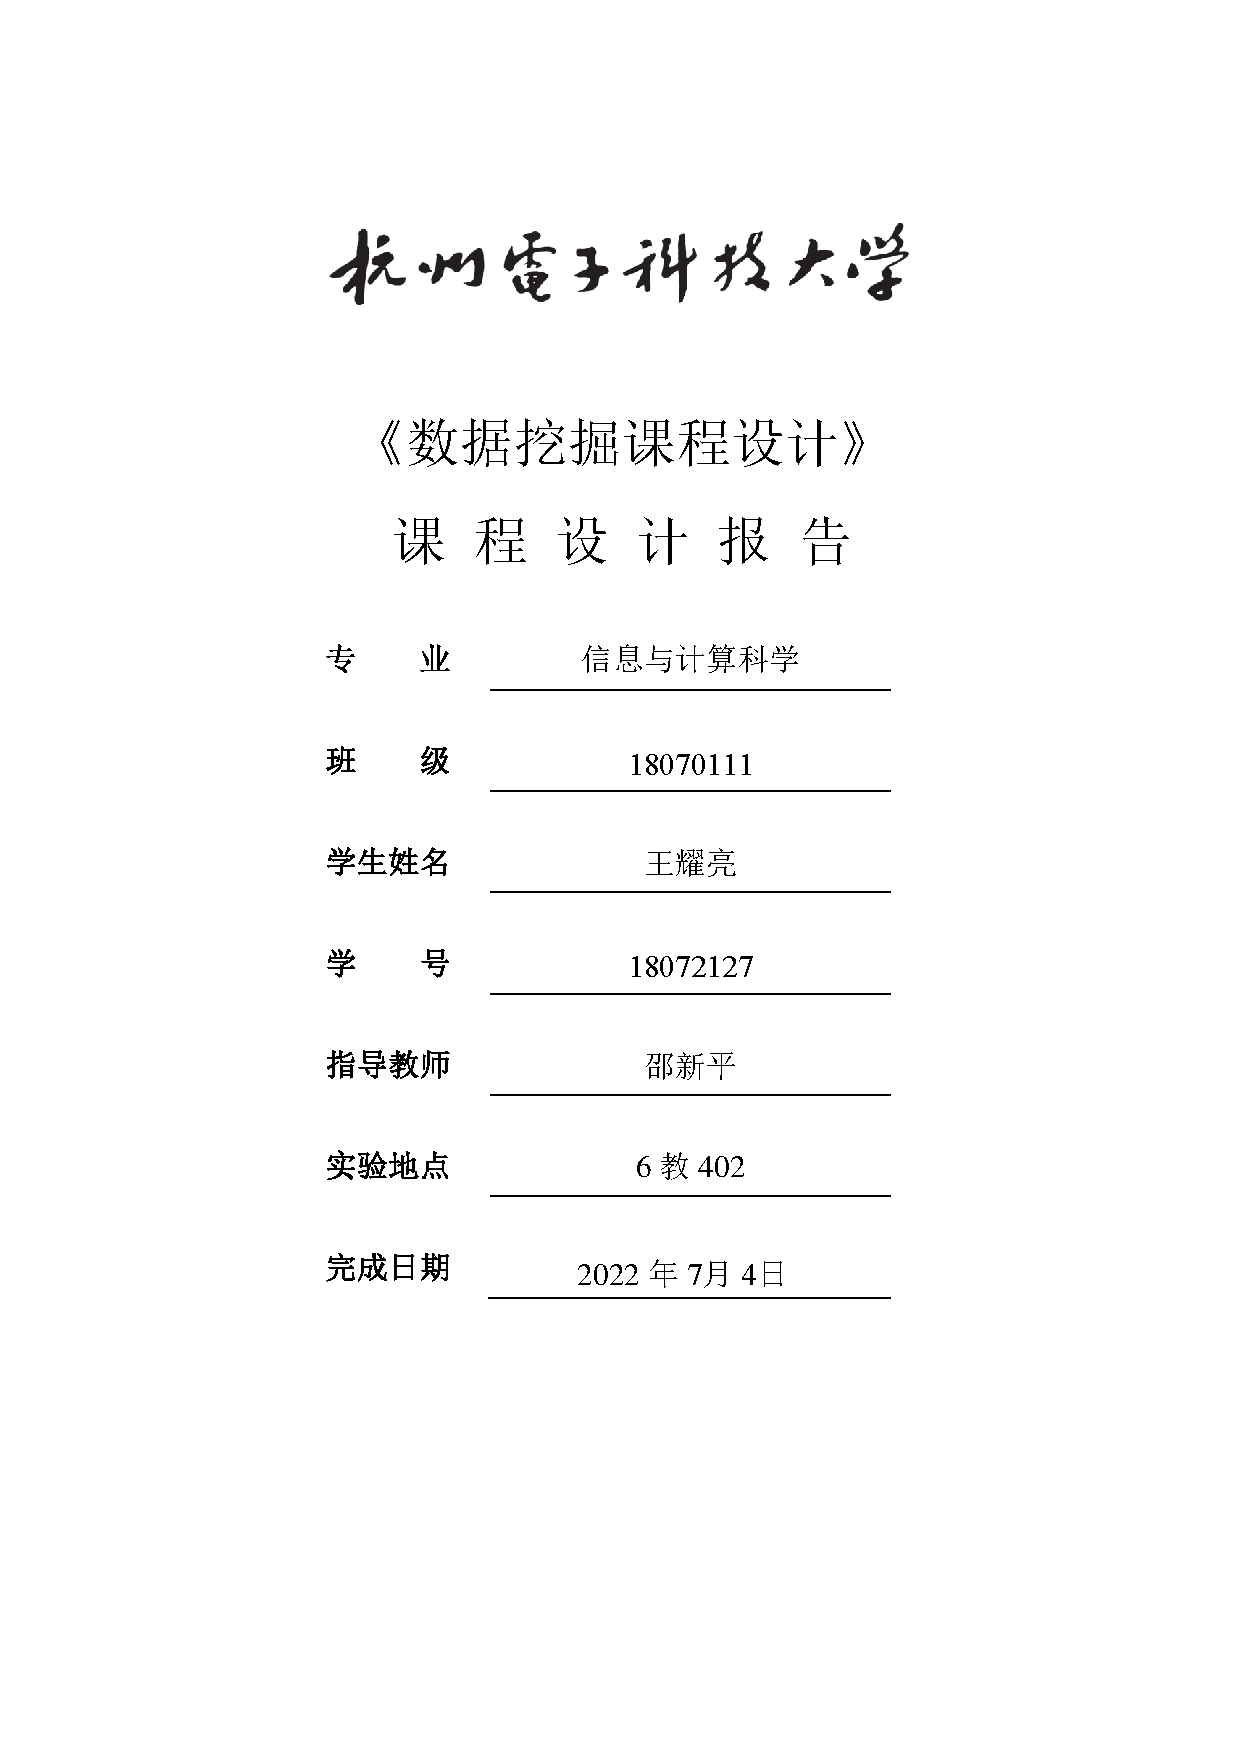
\includepdf{封面2.pdf} 
	\newpage
	
	%目录
	\tableofcontents
	
	\newpage
	\section{背景}
	\subsection{数据挖掘背景}
	\par 银行的主要收入来自贷款。但它往往与风险有关。借款人可能会拖欠贷款。为了缓解这个问题,银行决定使用机器学习来克服这个问题。他们收集了关于贷款借款人的过去数据,希望您开发一个强大的分类算法模型来分类是否有任何新的借款人可能违约。该数据集庞大,由多个决定性因素组成,如借款者的收入、性别、贷款用途等。
	
	\subsection{数据集介绍}
	\par 该数据集中有34个特征向量,DataFrame并没有显示所有特征向量。为了解决这个问题,我们可以使用pandas设置设置要显示的列数,如下单元格所示:
	
	\begin{lstlisting}
	pd.set_option("display.max_columns", dataset.shape[-1]) 
	dataset.head(5)
	\end{lstlisting}

	\begin{figure}[H]
		\centering
		\centerline{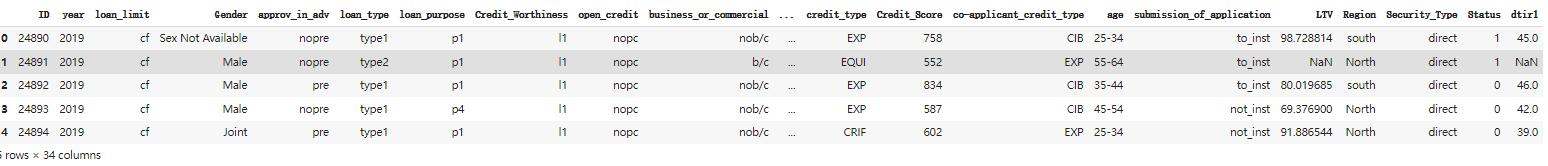
\includegraphics[width=\textwidth]{jie_2}}  
		\begin{center}
			\caption{数据集介绍}
		\end{center}
	\end{figure}
	
	\section{数据预处理}
	\par 数据预处理是准备原始数据并使其适合机器学习模型的过程。这是创建机器学习模型的第一步,也是至关重要的一步。在创建机器学习项目时,我们并不总是会遇到干净且格式化的数据。在对数据进行任何操作时,必须对其进行清理并以格式化的方式放置。为此,我们使用数据预处理任务.
	\par 真实世界的数据通常包含噪声、缺失值,并且可能是无法直接用于机器学习模型的不可用格式。数据预处理是清理数据并使其适合机器学习模型所需的任务,这也提高了机器学习模型的准确性和效率。数据预处理包括以下步骤:	
	\begin{itemize}
		\item 获取数据集
		\item 导入库
		\item 导入数据集
		\item 查找缺失数据
		\item 编码分类数据
	\end{itemize}
	
	\subsection{缺失值处理}
	\par 缺失数据在真实数据集中并不罕见。事实上,随着数据集大小的增加,至少一个数据点丢失的可能性增加。缺失数据可能以多种方式出现,在这里去,使用如下三种方法对缺失数据进行处理:
		\begin{itemize}
		\item 删除数据
		\item 编码缺失
		\item 插补方法
	\end{itemize}
	
	
	
			\begin{figure}[H]
		\centering
		\centerline{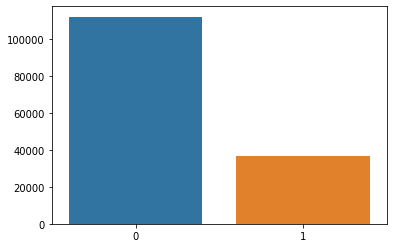
\includegraphics[width=0.4\textwidth]{jie_3}}  
		\begin{center}
			\caption{类1和类0分布}
		\end{center}
	\end{figure}
	
	
\section{多元线性回归}
\par 线性回归(linear regression)是试图学得一个线性模型以尽可能准确地预测实值的输出标记。线性回归一般被用在回归问题上,但是对线性回归做出简单的变换,即可用于进行二分类问题。此时的线性回归模型也就变成了我们熟悉的逻辑斯蒂回归(logistic regression)。而一个多分类问题又可以分解成多个二分类问题,于是我们同样可以将逻辑斯蒂回归模型用于解决多分类问题上。以下将顺序介绍线性回归,逻辑斯蒂回归,以及多分类问题如何分解成多个二分类问题。
\subsection{模型原理}
首先我们定义一下字符。一个样本我们用  x  来表示,数据集中第 $ \mathrm{k}$   个样本则为 $  x_{k}$   。一个样本中存在 $  \mathrm{d}$   个特征值,我们用一个列向量来表示 一个样本,即  $ x_{k}=\left(x_{k}^{1} ; x_{k}^{2} ; x_{k}^{3} ; \ldots ; x_{k}^{d}\right) $  。  w  是待学习的权重,因为每个样本中有 $  \mathrm{d} $  个特征,因此  $ \mathrm{w}$   是一个  $ \mathrm{d}$   维的列向量,记为  $ w=\left(w^{1} ; w^{2} ; w^{3}, \ldots, w^{d}\right) $  。在W和  $ \mathrm{b}$   确定的的情况下,模型就确定了下来  $ \hat{y}=w^{T} x+b$   。我们用均方误差来衡量模型的性能,则  $L(w,b)=\sum_{i=0}^{m}\left(y_{i}-\hat{y}_{i}^{2}\right)=\sum_{i=0}^{m}\left(y_{i}-w^{T} x_{i}-b\right)^{2} $  。其中m为样本总数。
简单梳理一下,在训练过程 (在这里我们把确定W和 $  \mathrm{b}$   的过程称为训练过程) 中我们的目标是找出令  $ L(w, b)=\sum_{i=0}^{m}\left(y_{i}-w^{T} x_{i}-b\right)^{2}$   最小的$   \mathrm{w} $  和  $ \mathrm{b} $  。而在测试过程(在这里我们把根据求得的 $  \mathrm{w}$   和  $ \mathrm{b}$   计算 $  \mathrm{y} $  的过程称为测试过程) 中,我们输入  x  的输出为  $ \hat{y}=w^{T} x+b $  。
目标明确后,我们如何计算得到  w  和  b  使得 $  \mathrm{L}(\mathrm{w}, \mathrm{b})$   最小. 因为这是一个线性模型,而且求解的目标是均方误差最小化,因此我们可以用最 小二乘法来求解W和  $ \mathrm{b}_{\text {。 }} $ 
p.s. 为了方便讨论,我们在下面的推导中将  x  的维度设为 1 ,即d  =1  首先将损失函数  L  分别对  w  和  b  求偏导,得:


\begin{align}
\frac{\partial L(w, b)}{\partial b}=-2 \sum_{i=1}^{m}\left(y_{i}-w x_{i}-b\right)
\end{align}


\begin{align}
\frac{\partial L(w, b)}{\partial w}=-2 \sum_{i=1}^{m}\left(x_{i} y_{i}-w x_{i}^{2}-b x_{i}\right)
\end{align}



令 $ \frac{\partial L(w, b)}{\partial b}=0    b=\frac{1}{m} \sum_{i=1}^{m}\left(y_{i}-w x_{i}\right) $ 又因为 $ m \bar{y}=\sum_{i=1}^{m} y_{i}, m \bar{x}=\sum_{i=1}^{m} x_{i} $ 所以

\begin{align}
w=\frac{\sum_{i=1}^{m} x_{i} y_{i}-\bar{y} \sum_{i=1}^{m} x_{i}}{\sum_{i=1}^{m} x_{i}^{2}-\bar{x} \sum_{i=1}^{m} x_{i}}=\frac{\sum_{i=1}^{m}\left(x_{i}-\bar{x}\right)\left(y_{i}-\bar{y}\right)}{\sum_{i=1}^{m}\left(x_{i}-\bar{x}\right)^{2}}
\end{align}










\subsection{相关系数矩阵}
\par 相关性热图测量数据集列之间的零相关性。它显示了一个特征的存在或不存在对另一个特征的影响有多大。
\begin{figure}[H]
\centering
\centerline{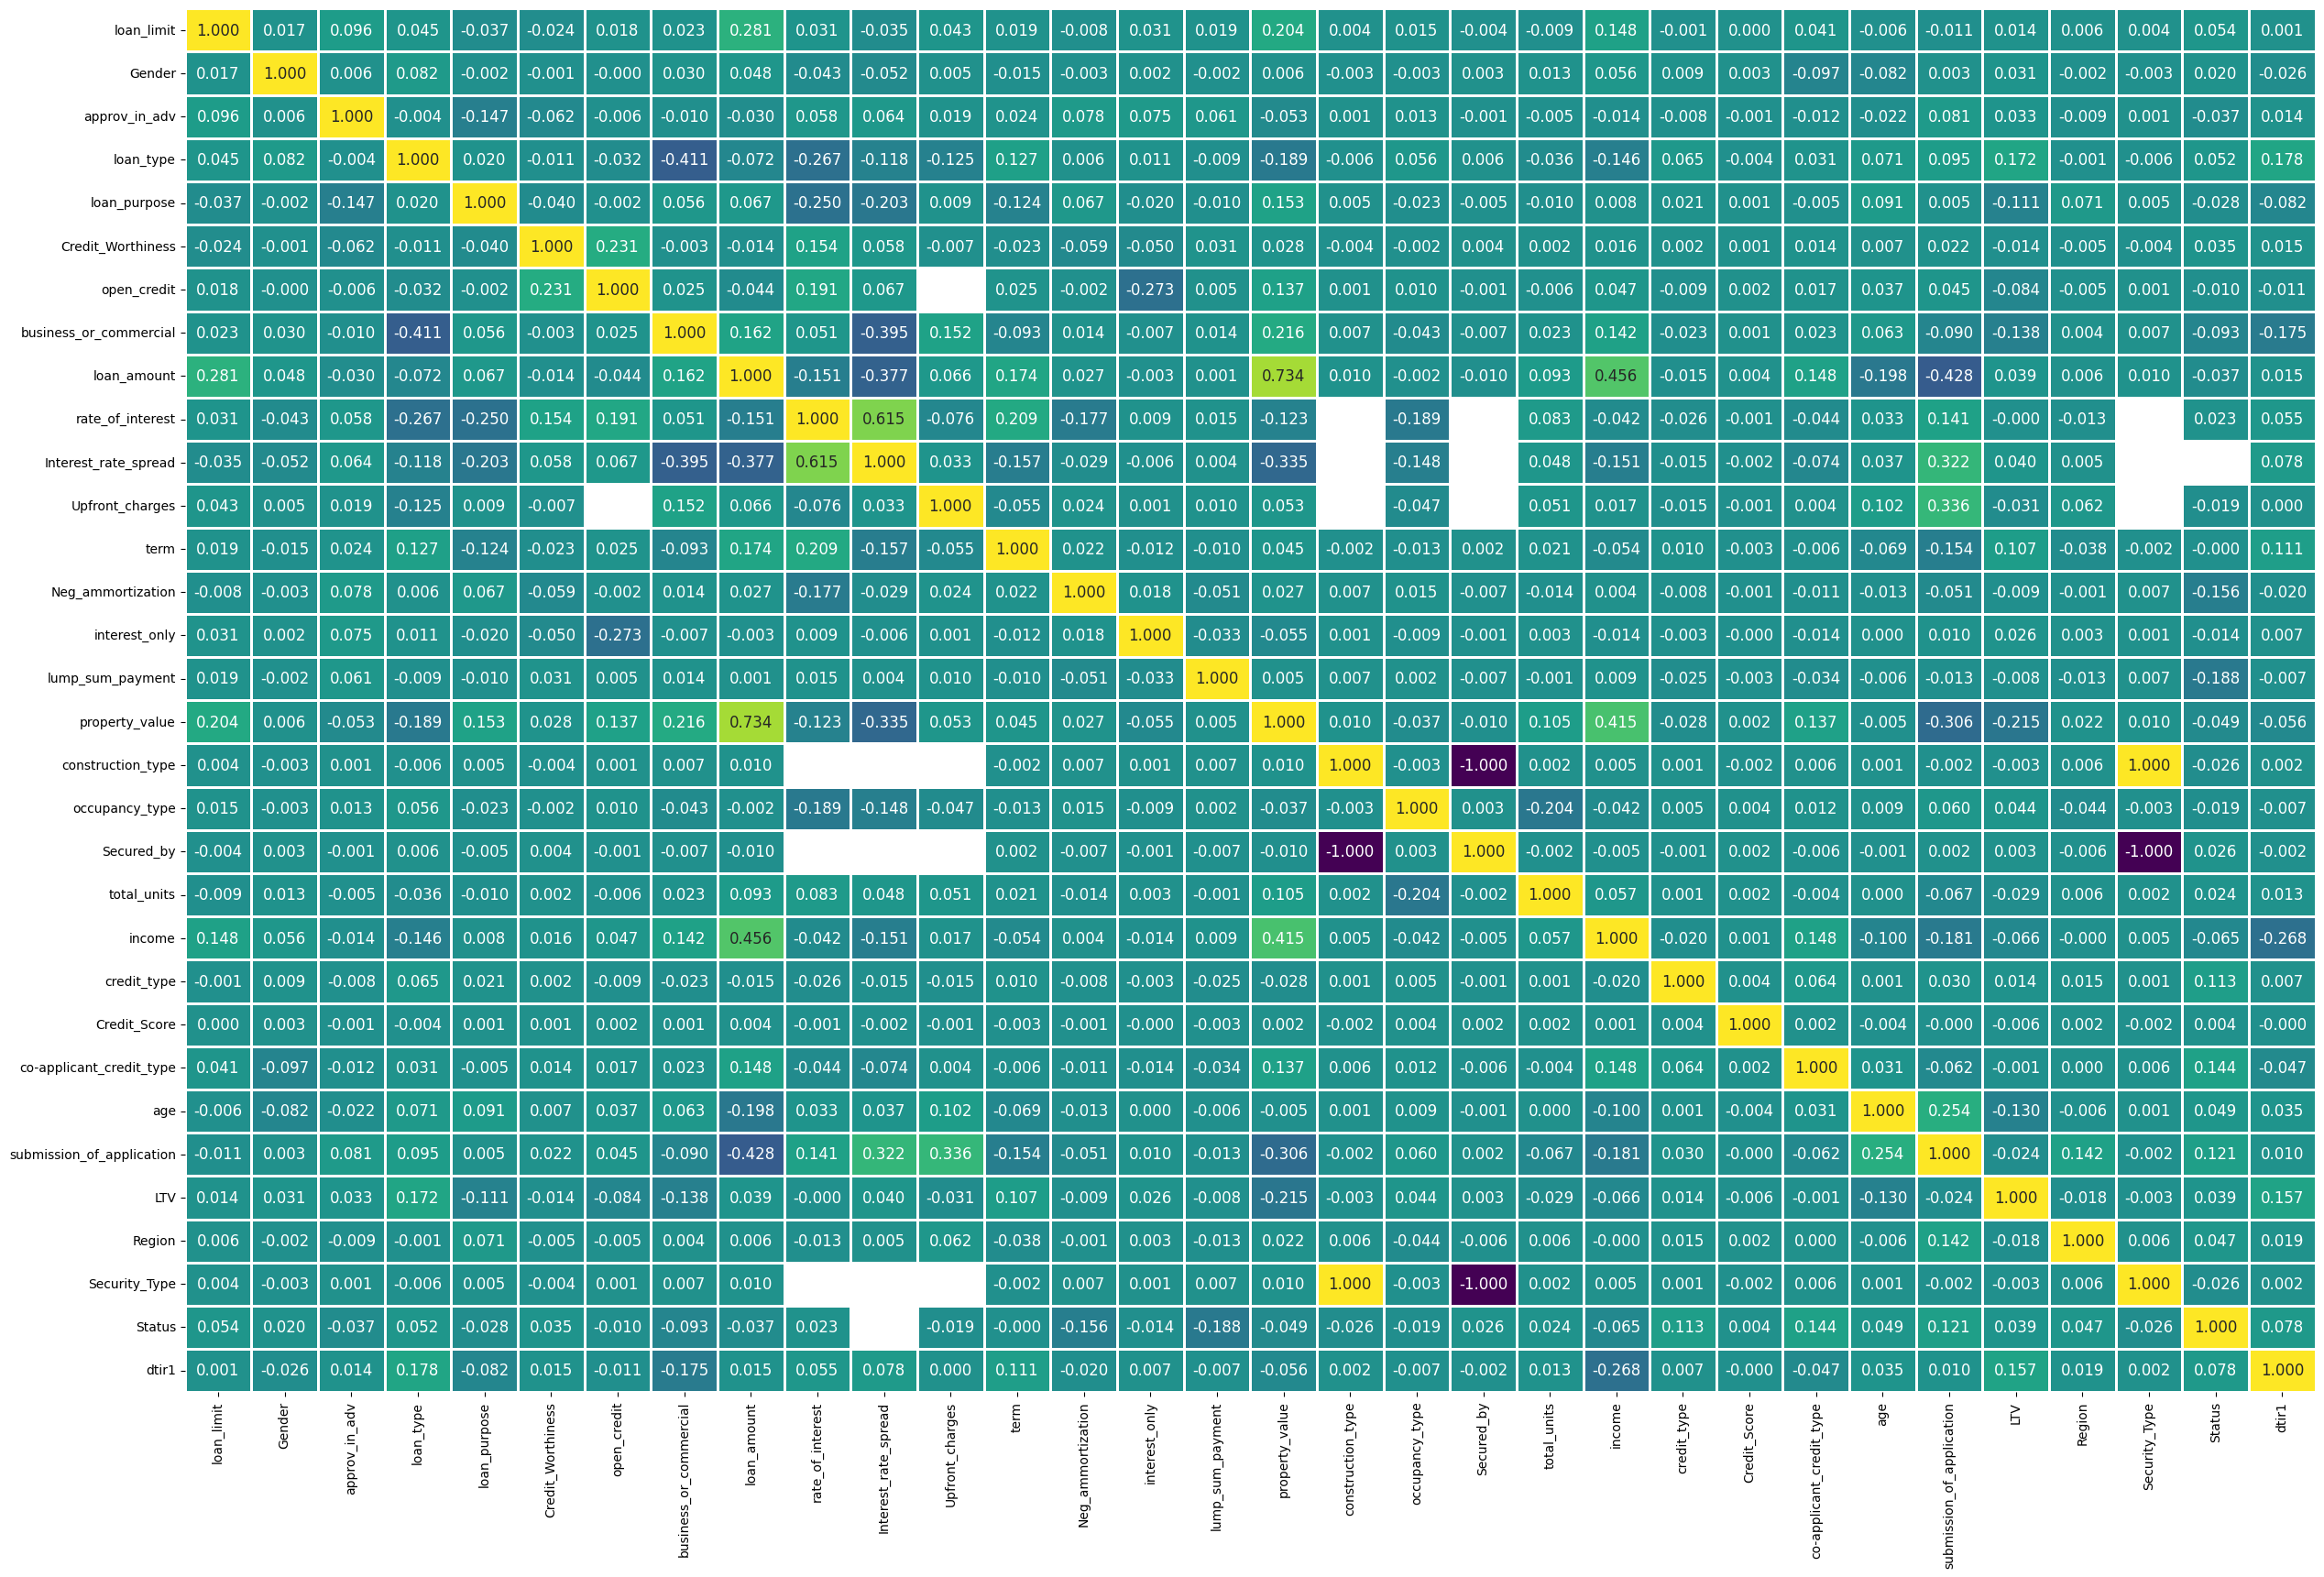
\includegraphics[width=0.9\textwidth]{jie_4}}  
\begin{center}
	\caption{相关系数矩阵}
\end{center}
\end{figure}

\par loan\_amount与property\_value为变量的散点图如下:
\begin{figure}[H]
	\centering
	\centerline{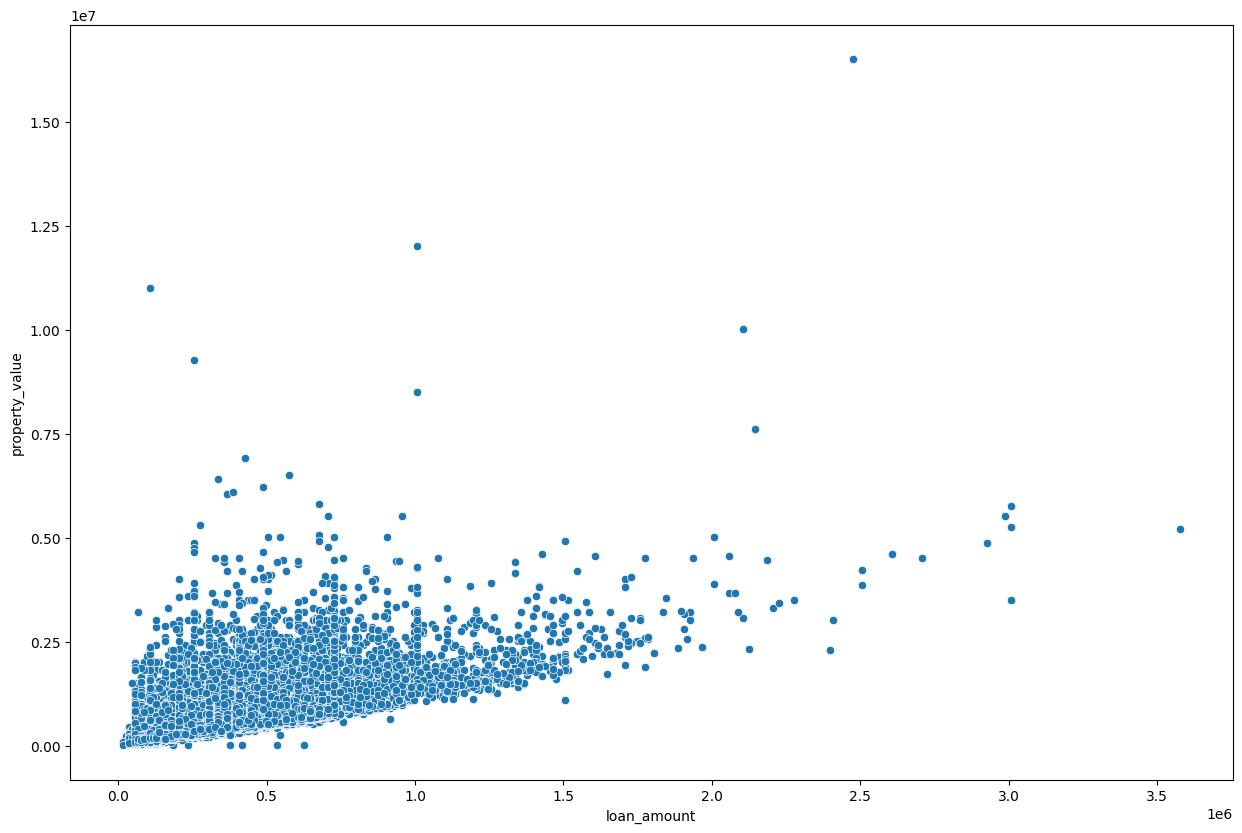
\includegraphics[width=0.5\textwidth]{jie_6}}  
	\begin{center}
		\caption{loan\_amount与property\_value散点图}
	\end{center}
\end{figure}
\par 从图中我们可以看到两个特征之间存在线性关系,但线性回归不能很好地拟合数据。虽然线性回归不能很好地拟合数据,但可以尝试使用线性回归,

\subsection{逻辑回归}
\subsubsection{模型原理}
\par 二分类问题: 对样本点 x, 其标签$y \in\{0,1\} $,想要知道的是概率
\begin{align}
	\operatorname{Pr}(y=1 \mid x)
\end{align}
\par 对于二分类问题,显然可以建模假设  $y \mid x$  服从参数为  p  的Bernoulli分布,因此只需要估计 $ p=E(y \mid x) $

\par Bernoulli分布是二项分布  n=1  的特殊情形,显然也属于指数分布族。使用GLM建模:选择Bernoulli分布  +  正规连接,得到
\begin{align}
	p=\frac{1}{1+e^{-\beta^{T} x}}=s\left(\beta^{T} x\right)
\end{align}


\par 其中  $s(\cdot)$  称为 Sigmoid 函数
\begin{align}
	s(z)=\frac{1}{1+e^{-z}}
\end{align}


\subsubsection{模型结果}
\par 使用逻辑回归得到的结果如下:
\begin{figure}[H]
	\centering
	\centerline{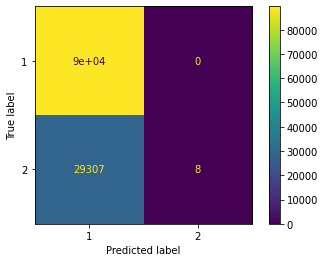
\includegraphics[width=0.5\textwidth]{jie_l_1}}  
	\begin{center}
		\caption{混淆矩阵}
	\end{center}
\end{figure}

\begin{figure}[H]
	\centering
	\centerline{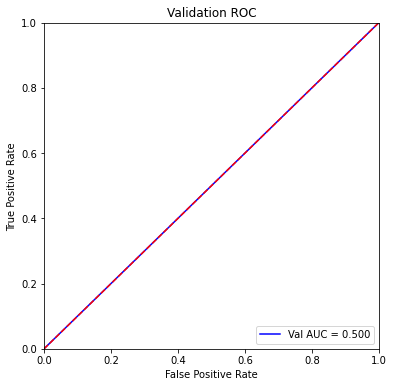
\includegraphics[width=0.5\textwidth]{jie_l_2}}  
	\begin{center}
		\caption{AUC曲线}
	\end{center}
\end{figure}

\par 可以看到,逻辑回归的AUC为0.5,效果很差。

\subsection{随机森林}
\subsubsection{模型原理}
\par  生成单棵决策树:
(1)训练总样本的个数为N,则单棵决策树从N个训练集中有放回的随机抽取n个作为此单颗树的训练样本。

(2)令训练样例的输入特征的个数为M,m远远小于M,则我们在每颗决策树的每个节点上进行分裂时,从M个输入特征里随机选择m个输入特征,然后从这m个输入特征里选择一个最好的进行分裂。m在构建决策树的过程中不会改变。这里注意,要为每个节点随机选出m个特征,然后选择最好的那个特征来分裂。

(3)每棵树都一直这样分裂下去,直到该节点的所有训练样例都属于同一类。不需要剪枝。由于之前的两个随机采样的过程保证了随机性,所以就算不剪枝,也不会出现over-fitting。


\subsubsection{模型结果}
\par 使用随机森林得到的结果如下:
\begin{figure}[H]
	\centering
	\centerline{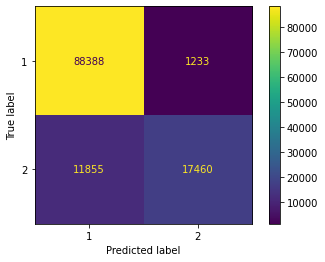
\includegraphics[width=0.4\textwidth]{jie_R_1}}  
	\begin{center}
		\caption{混淆矩阵}
	\end{center}
\end{figure}

\begin{figure}[H]
	\centering
	\centerline{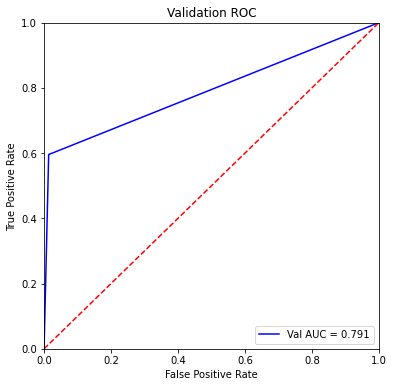
\includegraphics[width=0.4\textwidth]{jie_R_2}}  
	\begin{center}
		\caption{AUC曲线}
	\end{center}
\end{figure}

\par 可以看到,随机森林的AUC为0.791,效果比逻辑回归更好。



\end{document} 